\chapter{Complex event processing}
	\label{chap:cep}
	\section{Complex Event Processing with the current technologies}
		In the proposed hierarchical runtime verification approach, the top level of modelling and analysis is supported by a Complex Event Processing Framework.
		
		In our project we are going to do so, and define Event Patterns for the top level.
		Our choice for CEP is the VIATRA CEP, because it's the only open source CEP with 
		a live model integration, where you can define graph patterns to the model, and automatically generate atomic events
		on the appearance and disappearance of these patterns.
		
		VIATRA CEP uses a language called VIATRA Event Pattern Language, or VEPL for short.
		This language is perfect for our approach, it has a very simple syntax, and the event patterns can be defined in
		a very high level way, but the automaton which it translates the patterns to are not well-formalized, and the
		execution of the patterns are dependent on so called ``event contexts'' which makes the verification extremely hard.
		
		We propose an intermediate language, to which we can translate our patterns to. This language has to be 
		formalized.
		
		TODO abra : Harom doboz, High level -> Intermediate language (Regular Expressions) -> Executable code (Automatons)

		The operators of the language is show on \cref{tab:cep:veplop}. 
		The syntax sugars are shown on \cref{tab:cep:veplsugar},
		but we are going to ignore these, since they can be translated to the basic operators as show on \cref{tab:cep:veplsugartobasic}.
		
		We are going to introduce every step through an example, which is about the runtime verification of a two phase lock algorithm. %% TODO Reference
		In the two phase locking algorithm there are two rules :
		\begin{enumerate}
			\item Resources must be allocated in a previously defined sequence, which is the same for all tasks
			\item If a task releases a resource, it's not allowed to allocate anything anymore.
		\end{enumerate}
		
		Since this example uses resources, we have to define the following behaviour :
		Each resource can be allocated once before every release, and can be released once before every allocation.
		
		To further increase our effectiveness, we will define the following : The first phase must finish after 10 seconds,
		i.e. the time between the first allocation and the first release must be less than 10 seconds\footnote{In the final 
		example we are going to change this, to ``A resource cant be in allocated state for more than 10 sec'', but to 
		only have one automaton, we will use this rule right now.}.
		
			
		\begin{table}
		\caption{Basic operators}		
		\label{tab:cep:veplop}
		\begin{tabular}{lcm{6cm}}
		\centering
		Operator name &	Denotation & Meaning \\
		followed by & p1 $\rightarrow$ p2 & Both patterns have to appear in the specified order. \\
		or &	p1 OR p2 &	One of the patterns has to appear. \\
		``infinite'' multiplicity &	p\{*\} &	The pattern can appear 0 to infinite times. \\
		within timewindow &	p[t] &	Once the first element of the pattern is observed (i.e. the patterns ``starts to build up''), the rest of the pattern has to be observed within t milliseconds.
		\end{tabular}
		\end{table}

		\begin{table}
		\caption{Syntax sugars}		
		\label{tab:cep:veplsugar}
		\begin{tabular}{lcm{6cm}}
		\centering
		Operator name &	Denotation & Meaning \\
		and &	p1 AND p2 &	Both of the patterns has to appear, but the order does not matter.\\
		negation &	NOT p &	On atomic pattern: event instance with the given type must not occur. On complex pattern: the pattern must not match. \\
		multiplicity &	p\{n\} &	The pattern has to appear n times, where n is a positive integer.\\
		``at least once" multiplicity &	p\{+\} &	The pattern has to appear at least once. \\
		\end{tabular}
		\end{table}
		
		\begin{table}
		\caption{Syntax sugars mapped to basic operators}		
		\label{tab:cep:veplsugartobasic}
		\begin{tabular}{lcm{6cm}}
		\centering
		Operator name &	Denotation & Equivalent \\
		and &	p1 AND p2 & ((p1 $\rightarrow$ p2) OR (p2 $\rightarrow$ p1)). \\
		negation &	NOT $p$ & $\Sigma \setminus p$, where $\Sigma$ is the set of all the possible Events. \\
		multiplicity &	p\{n\} &	p1 $\rightarrow$ p1 $\rightarrow$ \dots p1, n times. \\
		``at least once" multiplicity &	p\{+\} & p $\rightarrow p\{\ast\}$ \\
		\end{tabular}
		\end{table}

		
	\section{Regular Expression}
		In this particular example, we need a language to describe event sequences. To do so, one of the most common
		formalism is a Regular Expression, where the alphabet is the set of possible events.
		
		\begin{dfn}
			(Left Derivate).\footnote{reference timed.pdf}
			For every two sequences $u$ and $v$ the left derivate of $u$ by $v$
			is a partial function defined as:
			%
			\[ v \setminus u
				\begin{cases}
					w & \text{ if } \exists w,u = vw \\
					\perp & \text{otherwise}
				\end{cases}
			\]
			%
			In other words, $v \setminus u$ is defined if $v$ is a prefix of $u$,
			and in that case $v$ is removed.
		\end{dfn}
		
		\begin{dfn}
			(Absorbing concatenation).
			The partial operator $u \circ v$ on $\mathcal{T}$ is defined as:
			\[ u \circ v = u \cdot (\lambda (u) \setminus v) \]
		\end{dfn}
		
		\begin{dfn}
			\label{dfn:cep:re}
			Regular Expressions over an alphabet $\Sigma$ (also referred to as $\Sigma$-expressions)
			are defined using the following families of rules.
			\begin{enumerate}
				\item \underline{$a$} for every letter $a \in \Sigma$ and the special symbol $\varepsilon$ are expressions.
				\item If $\varphi, \varphi_1, \varphi_2$ are $\Sigma$-expressions then %
					$ %
					\varphi_1~\cdot~\varphi_2,
					\varphi_1 \vee \varphi_2,
					\varphi_1 \circ \varphi_2,
					\varphi_1 \wedge \varphi_2,
					\varphi^\ast,
					\varphi^\circledast
					$ are $\Sigma$-expressions.
			\end{enumerate}
		\end{dfn}
		
		Using Regular Expressions we can describe an event sequence as $ab$, if $a,b \in \Sigma$ and the meaning of this is that ``an $a$ event will happened,
		and a $b$ event will follow it''. In the two phase locking example we are going to describe the behaviour of one resource with a simple VEPL pattern:
		$(a \rightarrow f)\{\ast\}$ which means that an infinite sequences of allocation and release are allowed after each other. This is equivalent to the 
		regular expression : $(af)\ast$.

		\subsection{Deterministic Finite Automaton}
			To match Regular Expressions, the most common solution is to make an automaton, there are many algorithms for this.  %% TODO Reference?
			
			
			\begin{dfn}
				\label{dfn:cep:dfea}
				An Event Automaton (Deterministic Finite Event Automaton in other words) is a $\langle Q,\Sigma,\delta_d,q_0, F \rangle$ tuple where: 
					\begin{itemize}
						\item $Q$ is a finite, non empty set. These are the states of the automaton,
						\item $\Sigma$ is a finite, non empty set. This is the Event set of the automaton,
						\item $\delta_d$ is a set of $\langle Q \times \Sigma \times Q \rangle$ tuples,
							and the number of outgoing edges from each state for each event is only one 
							i.e. $\forall q_0 \in Q$ and $\forall e_0 \in \Sigma$ : $|\langle q_0, e_0, q_1 \rangle| = 1$, where $q_1 \in Q$ 
						\item $q_0 \in Q$ a start state,
						\item $F \subseteq Q$ the set of the acceptor states.
					\end{itemize}	
			\end{dfn}

			The semantic is the following : 
			On input $e$, where $e \in \Sigma$, if the token is on State $s$ the next state will be $s'$ where % TODO Remove token from semantics
			$\delta_d \langle s,e,s' \rangle$. For short, from now we will use $s \rightarrow s'$ to shorten this. 
			
			The regular expression of the example can be compiled to this automaton\footnote{TODO ide kell egy abra a resource automatajarol}:
			
			

		
	\section{Timed Regular Expression}
	
		With the previously defined semantics we can not express temporal statements,
		but regular expressions can be expanded to a formalism which can do so : 
		the Timed Regular Expressions
		

		\begin{dfn}
			\label{dfn:cep:tre}
			Timed Regular Expressions over an alphabet $\Sigma$ (also referred to as $\Sigma$-expressions)
			are defined using the following families of rules~\citep{tre}~.
			\begin{enumerate}
				\item \underline{a} for every letter $a \in \Sigma$ and the special symbol $\varepsilon$ are expressions.
				\item If $\varphi, \varphi_1, \varphi_2$ are $\Sigma$-expressions and $I$ is an integer-bounded interval then
					$\langle\varphi\rangle_I, \varphi_1~\cdot~\varphi_2, \varphi_1 \vee \varphi_2,$ and $\varphi^\ast$ are $\Sigma$-expressions.
				\item If $\varphi, \varphi_1$ and $\varphi_2$ are $\Sigma$-expressions then $\varphi_1 \circ \varphi_2, \varphi^\circledast$ are
					$\Sigma$-expressions.
				\item If $\varphi_1$ and $\varphi_2$ are $\Sigma$-expressions, $\varphi_0$ is a $\Sigma_0$-expression
					for some alphabet $\Sigma_0$, and $\Theta$ : $\Sigma_0 \rightarrow \Sigma$ is
					a renaming, then $\varphi_1 \wedge \varphi_2$ and $\Theta(\varphi_0)$ are $\Sigma$-expressions.
			\end{enumerate}
		\end{dfn}
		
		\subsection{Timed Event Automaton}
			\begin{dfn}
				\label{dfn:cep:tea}
				A Timed Event Automaton $\langle Q,\Sigma,\delta,q_0, F, t, T \rangle$ where
				\begin{itemize}
					\item $Q, \Sigma, q_0,$ and $F$ are the same as in Definition \ref{dfn:cep:ea},
					\item $t$ is a global clock variable $t \in \mathbb{R}$,
					\item $T$ is a set of local timeout clocks, i.e. a set of tuples $\langle Q, \RR \rangle$
					\item and $\delta$ is the union of discrete and timed transitions i.e. $\delta_t \cup \delta_d$ where
					\begin{itemize}
						\item $\delta_d$ is defined as in Definition \ref{dfn:cep:ea},
						\item and $\delta_t$ represents timed transitions and defined as the set of tuples $\langle Q \times \mathbb{R} \times Q \rangle$ 
					\end{itemize}
				\end{itemize}
			\end{dfn}
			
			The semantic of the Timed Deterministic Finite Automaton is defined as follows:
			
			
			
			$Q_t \subseteq Q$ is the set of states with outgoing timed transitions, 
			i.e. $\forall s \in Q_t$ : there exist $ \delta_t\langle s, t, s' \rangle$ where $t \in \RR$ and $s' \in Q$.
			We have to define rules for entering states with timed outgoing transitions and we also define the general rules of changing states. 
			
			\begin{enumerate}
				\item Initialization Rule : On initialization of the automaton, we have to set all clocks to $\infty$ 
				i.e. $\forall t_i \forall q_i T \langle q_i, t_i \rangle, t_i \coloneqq \infty $
				
				\item Entering Timed State Rule: On entry to state $s$ where $s \in Q_t$ the timeout variable $t_s$ of the state is set according to the value of the global time and the timeout value of the output transition $t_{timeout}$:
					$t_s\coloneqq t+t_{timeout}$
					where $T\langle s,t_s \rangle$ and $\delta_t\langle s,t_{timeouts},s' \rangle$ where $t_{timeout}$ is minimal from the set of possible $t_{timeouts}$ 
				
				\item Firing Transitions Rule: Non deterministically choose an enabled transition from the set of enabled discrete or timed transitions. 
					$s$ is the state we currently in, and $s'$ is the state we are moving to.
					We have two cases, the chosen transition is:
					\begin{enumerate}
						\item Discrete Transition: In case of $s' \notin Q_t$ than the execution of the transition is as in described formerly. 
						If we exit state $s \in Q_t$ by a transition in $\delta_d$, 
						then the following rule extends the firing rule of discrete transitions by invalidating the corresponding timeout values:
							$t_s \coloneqq \infty$, where $T \langle t_s, s \rangle$
						\item Timed Transition: The transition with the minimal timeout value is selected, 
							i.e. transition $\delta_t$ from state $s_t$ where $\forall q \in Q_t: t_q \geq t_s$, than the following rules apply:
							the global time is set $t \coloneqq t_s$, the local clock is set to infinity: 
							$t_s \coloneqq \infty$ and move to through $\delta_t : s \rightarrow s'$ the next state according to $\delta_t$.
					\end{enumerate}			
			\end{enumerate}
		
		\subsection{Timed Region Automaton}
			\begin{dfn}
				\label{dfn:cep:TREA}
				A Timed Region Event Automaton $\langle Q,\Sigma,\delta,q_0, F, t, T \rangle$ where
				\begin{itemize}
					\item $Q, \Sigma, q_0, F,$ and  $t$ are the same as in Definition \ref{dfn:cep:tea},
					\item $T$ is a set of timeout clocks for sets of states, i.e. a set of tuples $\langle 2^Q, \RR \rangle$
					\item and $\delta$ is the union of discrete and timed transitions i.e. $\delta_t \cup \delta_d$ where
					\begin{itemize}
						\item $\delta_d$ is defined as in Definition \ref{dfn:cep:dfea},
						\item and $\delta_t$ represents timed transitions and defined as the set of tuples $\langle 2^Q , \mathbb{R} , Q \rangle$ 
					\end{itemize}
				\end{itemize}
			\end{dfn}
			
			The semantic of the Timed Region Automaton is defined as follows:
			$Q_t \subseteq Q$ is the set of states with outgoing timed transitions, 
			i.e. $\forall q \in Q_t$ : there exist $ \delta_t\langle s, t, s' \rangle$ where $t \in \RR$ and $s' \in Q$.
			Let us use the following notations: 
		
			$s$ is the state we are currently on, and $s'$ is the state we move to after the transition
		
			$r$ is the set of zones we are currently in, 
			i.e. $r \subseteq 2^Q$ where $\exists r_s : r_s \in r, s \in r_s $ 
			
			$r'$ is the set of zones we enter,
			i.e. $r \subseteq 2^Q$ where $\exists r_s :  r_s \in r, s' \in r_s $ 
			
			$r^+ \subseteq 2^Q$ is a set of new timed regions we just entered,
			i.e. $r^+ = r' \setminus r$ 
			
			$r^- \subseteq 2^Q$ is a set of timed zones we just left
			i.e. $r^- = r \setminus r'$
		
			We have to define rules for the initialization of the automaton,
			entering states with timed outgoing transitions 
			and we also define the general rules of changing states. 
			
			\begin{enumerate}
				\item Initialization Rule : On initialization of the automaton, we have to set all clocks to $\infty$ 
				i.e. $\forall t_i, \forall q_i, T \langle r_i, t_i \rangle, t_i \coloneqq \infty $, where $r_i \in 2^Q$
			
				\item Entering new timed region rule :
				If we enter a new set of timed regions, 
				i.e. $r^+ \neq \emptyset$, 
				we set the timers according to the timeouts, 
				i.e. $\forall t_{timeout} : t_{timeout} \coloneqq t + t_i $ where $ r_t \in r^+, \exists q ,\delta_t\langle  r_t,t_i,q \rangle, T \langle r_t, t_{timeout} \rangle$
				
				\item Firing Transitions Rule: Choose an enabled transition from the set of enabled\footnote{non defined} discrete or timed transitions. 
				We have two cases, the chosen transition is:
					\begin{enumerate}
						\item Discrete Transition: In case of $r^- = \emptyset$ than the execution of the transition is as in described formerly. 
							If else if we exit a zone i.e. $r^- = \emptyset$, 
							then the following rule extends the firing rule of discrete transitions:
							$\forall t_s, \forall q_s$ in $ \delta_t \langle r_i, t_s, q_s \rangle$ where $r_i \in r^-$, the timer of the regions are invalidated i.e.
							$t_s \coloneqq \infty$
						\item Timed Transition: The transition with the minimal timeout value is selected, 
							 i.e. transition $\exists t_i, \exists s_i, \delta_t \langle r_i, t_i, s_i \rangle$ where $ r_i \in r$ and $t_{min}$ is the minimum from all $t_i$,
							 than the following rules apply:
							 the global time is set $t \coloneqq t_{min}$, the local clock is set to infinity: $t_s \coloneqq \infty$ and move to the next state according to $\delta_t$.
					\end{enumerate}			
			\end{enumerate}


		
	\section{Parametric Timed Regular Expression}
		To process event from multiple source from the same type, as we need to do so in the example (There are multiple tasks and resources with the same behaviour),
		we can extend our formalism towards the parametric 
		
		\begin{dfn}
		A Parametric Timed Regular Expression is \dots %TODO
		\end{dfn}
	
		\subsection{Parametric Timed Region Automaton}
			
			
			We use $s$ to denote a tuple $\langle s_0,\dots,s_k \rangle$. We use $X \rightarrow Y$ and $\rightharpoondown$ to denote sets of total and partial function between
			$X$ and $Y$, respectively. We write maps (partial functions) as $[x_0 \mapsto v_0,\dots,x_i \mapsto v_i]$ and the empty maps as $[]$. Given two maps $A$ and $B$,
			the map override operator is defined as:
				\[
				 (A \dagger B)(x) = 
				  \begin{cases} 
				   B(x) & \text{if } x \in \text{\underline{dom}(B)} \\
				   A(x) & \text{if } x \notin \text{\underline{dom}(B)} \text{ and } x \in \text{\underline{dom}(A)} \\
				   \text{undefined otherwise.}
				  \end{cases}
				\]
 			
			\begin{dfn}
				(Smybols, Events, Alphabets and Traces).
				Let $\mathit{Sym} = \mathit{Val} \cup \mathit{Var}$ be the set of all symbols (variables or values).
				An event is a pair $\langle e, \overline{s} \rangle \in \Sigma \times \mathit{Sym}^\ast,$ written $e(\overline{s})$.
				An event $e(\overline{s})$ is ground if $\overline{s} \in \mathit{Val}^\ast$.
				Let Event be the set of all events and GEvent be the set of all ground events.
				A trace is a finite sequence of ground events.
				Let Trace = $GEvent^\ast$ be the set of all traces
			\end{dfn}
			
			\begin{dfn}
				(Substitution).
				The binding $\theta = [x_0 \mapsto v_0, \dots, x_i \mapsto v_i]$ can be applied to a symbol $s$ and to an event
				$e(\overline{s})$ as follows: 
				\[
				 s(\theta) = 
				  \begin{cases} 
				   \theta(s) & \text{if } s \in \underline{dom}(\theta) \\
				   s & \text{otherwise}
				  \end{cases}
				  \qquad e \langle s_0,\ldots,s_j \rangle (\theta) = e \langle s_0(\theta),\ldots,s_j(\theta) \rangle
				\]
			\end{dfn}
			
			\begin{dfn}
				(Matching).
				Given a ground event a an event b the predicate matches (a, b) hold if there exists a binding $\theta$ s.t. b($\theta$) = a.
				Moreover let match(a,b) denote the smallest such binding w.r.t $\sqsubseteq$ if it exists (and is undefined otherwise)
			\end{dfn}
			
			\begin{dfn}
				(Configurations and Transition Relation).
				We define configurations as elements o the set Config = Q $\times$ Bind. Let $\rightarrow \subseteq$ Config $\times$ GEvent $\times$ Config be a relation on
				configurations s.t. configurations $\langle q, \varphi \rangle$ and $\langle q', \varphi' \rangle$ are related by the ground event a, written
				$\langle q, \varphi \rangle \xrightarrow{\text{a}} \langle q' \varphi' \rangle$ if, and only if
					\begin{align}
						\exists b \in \mathcal{A}, & \exists \gamma \in Assign : (q, b, \gamma, q') \in \delta \wedge \\
						&matches(a,b) \wedge \varphi' = \gamma(\varphi \dagger match(a,b))
					\end{align}
				Let the transition relation $\rightarrow_{E}$ be the smallest relation containing $\rightarrow$ such that for any event
				$a$ and configuration $c$ if $\nexists c' : c \xrightarrow{\text{a}} c'$ then $ c \xrightarrow{\text{a}}_E c$.
				The relation $\rightarrow_E$ is lifted to traces.
				For any two configurations $c$ and $c'$, $ c \xrightarrow{\text{$\epsilon$}}_E c$ holds, and $\xrightarrow{\text{a.$\tau$}}_E c'$ holds
				if there exist a configuration $c'$ s.t. $c \xrightarrow{\text{a}}_E c'' \xrightarrow{\text{$\tau$}}_E c'$
			\end{dfn}
			
			
			\begin{dfn}
				\label{dfn:cep:PTREA}
				A Parametric Timed Region Event Automaton $\langle Q,\Sigma,\delta,q_0, F, t, T \rangle$ where
				\begin{itemize}
					\item $Q, \Sigma, q_0, F,$ and  $t$ are the same as in Definition \ref{dfn:cep:tea},
					\item $T$ is a set of timeout clocks for sets of states, i.e. a set of tuples $\langle 2^Q, \RR, B \rangle$, where $B$ is a binding
					\item and $\delta$ is the union of discrete and timed transitions i.e. $\delta_t \cup \delta_d$ where
					\begin{itemize}
						\item $\delta_d$ is defined as in Definition \ref{dfn:cep:dfea},
						\item and $\delta_t$ represents timed transitions and defined as the set of tuples $\langle 2^Q \times \mathbb{R} \times Q \rangle$ 
					\end{itemize}
				\end{itemize}
			\end{dfn}

			
		
		PRE REFACTOR. PRE REFACTOR. PRE REFACTOR. PRE REFACTOR. PRE REFACTOR. PRE REFACTOR. PRE REFACTOR. PRE REFACTOR. PRE REFACTOR. PRE REFACTOR. PRE REFACTOR. PRE REFACTOR. 
		After this comment, the whole chapter is obsolete, must rewrite it.
	
				
			\begin{dfn}
				(Parametric Timed Region Automaton).
				PTRA$\langle Q, \Sigma, \delta, f_0, F, t, T \rangle$
				\begin{itemize}
					\item where $\delta = \delta_t \cup \delta_d$
					\item and $Q, \Sigma, \delta_d, f_0, F$ and $t$ are defined as in Definition \ref{dfn:cep:TEA}
					\item $\delta_t \langle R, Q, \RR \rangle $ where $R \subseteq 2^Q$
					\item $T\langle R, B, \RR \rangle$ where $B$ is a set of binding and  $R \subseteq 2^Q$

				\end{itemize}
				
			\end{dfn}
			
			The semantic of the Parametric Timed Region Automaton is defined as follows:
			$Q_t \subseteq Q$ is the set of states with outgoing timed transitions, i.e. $\forall s \in Q_t$ : there exist $ \delta_t\langle r, t, s' \rangle$ where $t \in \RR$ and $s' \in Q$, and $r \subseteq 2^Q$ and $s \in r$
			
			$s$ is the state we are currently in, $s'$ is the state we move the token to.
			
			$r^+$ is the new regions we enter, i.e. $ r_i \setminus r_j $ where $ \exists r_i \exists k_i \exists q_i \delta_t\langle r_i,k_i,q_i \rangle$ and $ r_i \setminus r_j $ where $ \exists r_j \exists k_j \exists q_j \delta_t\langle r_j,k_j,q_j \rangle$ and $ s \in r_i$ and $s' \in r_j$.
			
			$r^-$ is the old regions we leave, i.e. $ r_j \setminus r_i $.
			%%TODO rewrite the semantics
			We have to define rules for entering states with timed outgoing transitions and we also define the general rules of changing states. 
			\begin{enumerate}
				\item Initialization Rule : On initialization of the automaton, we have to set all clocks to $\infty$ 
					i.e. $\forall t_i in \delta_t \langle q_i, t_i \rangle where \exists q_i$ and $t_i \coloneqq \infty $
			
				\item Entering Timed Region Rule: On entry to state $s'$ we calculate $r^+$, and start every timer.
					i.e. $\forall t_i$ in $\delta_t\langle r, s', t_i \rangle$  
				
				
					where $s \in Q_t$ the timeout variable $t_s$ of the state is set according to the value of the global time and the timeout value of the output transition $t_{timeout}$:
					$t_s\coloneqq t+t_{timeout}$ %\TODO
					where $T\langle s,t_s \rangle$ and $\delta_t\langle s,t_{timeouts},s' \rangle$ where $t_{timeout}$ is minimal from the set of possible $t_{timeouts}$ 
				
				\item Firing Transitions Rule: Deterministically choose an enabled transition from the set of enabled discrete or timed transitions. We have two cases, the chosen transition is:
					\begin{enumerate}
						\item Discrete Transition: In case of $s \notin Q_t$ than the execution of the transition is as in described formerly. If we exit state $s \in Q_t$ by a transition in $\delta_d$, 
						then the following rule extends the firing rule of discrete transitions:
							$t_s \coloneqq \infty$
						\item Timed Transition: The transition with the minimal timeout value is selected, i.e. transition $\delta_t$ from state $s_t$ where $\forall q \in Q_t: t_q \geq t_s$, than the following rules apply:
						 the global time is set $t \coloneqq t_s$, the local clock is set to infinity: $t_s \coloneqq \infty$ and move to the next state according to $\delta_t$.
					\end{enumerate}			
			\end{enumerate}
				
	\section{Examples of Event Processing}
 
 
		\subsection{File System}
			\subsubsection{Problem}
				File system - A file shouldn't be read when it has been opened for writing, and shouldn't be written, when opened for reading. 
				A file shouldn't be opened for writing and reading without a close event between the two different opens~\citep{marq}.
				The possible parametrized events are : 
				Open(file, mode), 
				Close(file), 
				Read(file), 
				Write(file). 
				Mode is either "R" or "W" which stands for Read and Write respectively.
			\subsubsection{Solution}
				We are looking for these patterns :

				\begin{itemize}
					\item open(f,"W") $\rightarrow$ NOT close(f)$\{\ast\}$ $\rightarrow$ open(f,"R");
					\item open(f,"R") $\rightarrow$ NOT close(f)$\{\ast\}$ $\rightarrow$ open(f,"W");
					\item open(f,"W") $\rightarrow$ NOT close(f)$\{\ast\}$ $\rightarrow$ read(f);
					\item open(f,"R") $\rightarrow$ NOT close(f)$\{\ast\}$ $\rightarrow$ write(f);
				\end{itemize}

				These event patterns can be matched with the automaton seen on \cref{fig:cep:fileautomaton}
				
				\begin{figure}[h]
				\centering
				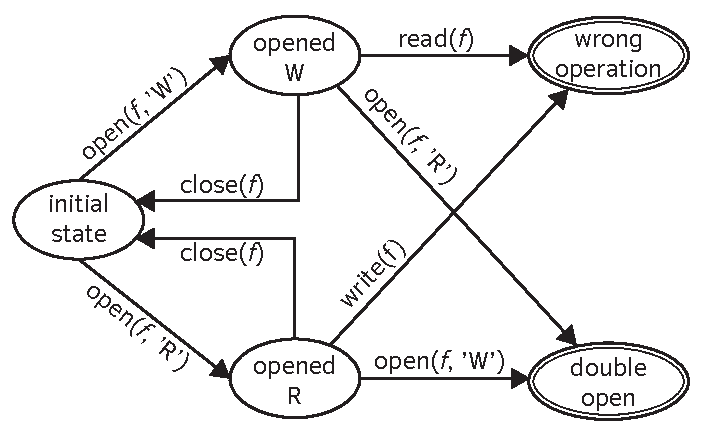
\includegraphics[width=0.7\linewidth]{include/figures/chapter_5/file_example_aut}
				\caption{Automaton of the file example}
				\label{fig:cep:fileautomaton}
				\end{figure}

		
		
		\subsection{Mars Rover Tasking - Two phase locking}
			\subsubsection{Problem}
				In concurrent systems the avoidance of deadlocks and livelocks are an utmost importance.
				To solve this problem, one of the many patterns is  the two phase locking - which can be defined by two rules.
				These rules are : 
				\begin{enumerate}
					\item \label{itm:cep:mp1} Every task must allocate the resources in a given order.
					\item \label{itm:cep:mp2} If a task releases a resource, it can't allocate anymore
				\end{enumerate}
			\subsubsection{Solution}
				Since our implementation doesn't support guards \emph{yet} we can only use constant amount of resources.
				For this example, this amount will be set to two, to minimize the model of the example.
				The \cref{itm:cep:mp1} pattern can be matched with the \cref {fig:cep:marsautomaton1}, and the \cref{itm:cep:mp2} 

				\begin{figure}[h]
				\centering
				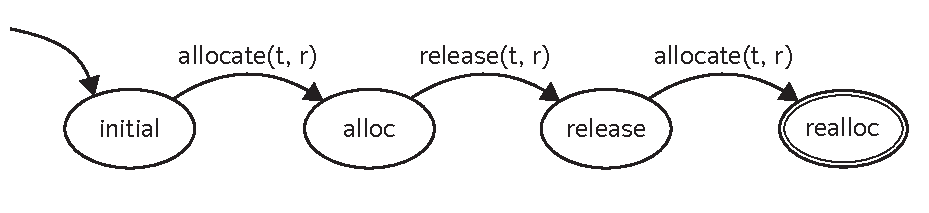
\includegraphics[width=0.7\linewidth]{include/figures/chapter_5/mars_example_aut1}
				\caption{Automaton to forbid the reallocation}
				\label{fig:cep:marsautomaton1}
				\end{figure}		
				
				
				\begin{figure}[h]
				\centering
				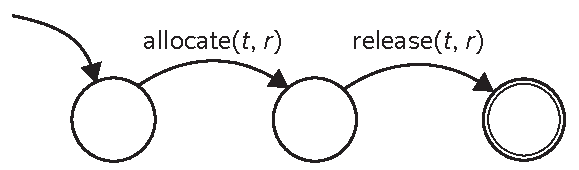
\includegraphics[width=0.7\linewidth]{include/figures/chapter_5/mars_example_aut2}
				\caption{Automaton to forbid inverse allocation}
				\label{fig:cep:marsautomaton2}
				\end{figure}	

				
				
	\section{Implementation}
		\subsection{Metamodel}
		
			\begin{figure}[h]
			\centering
			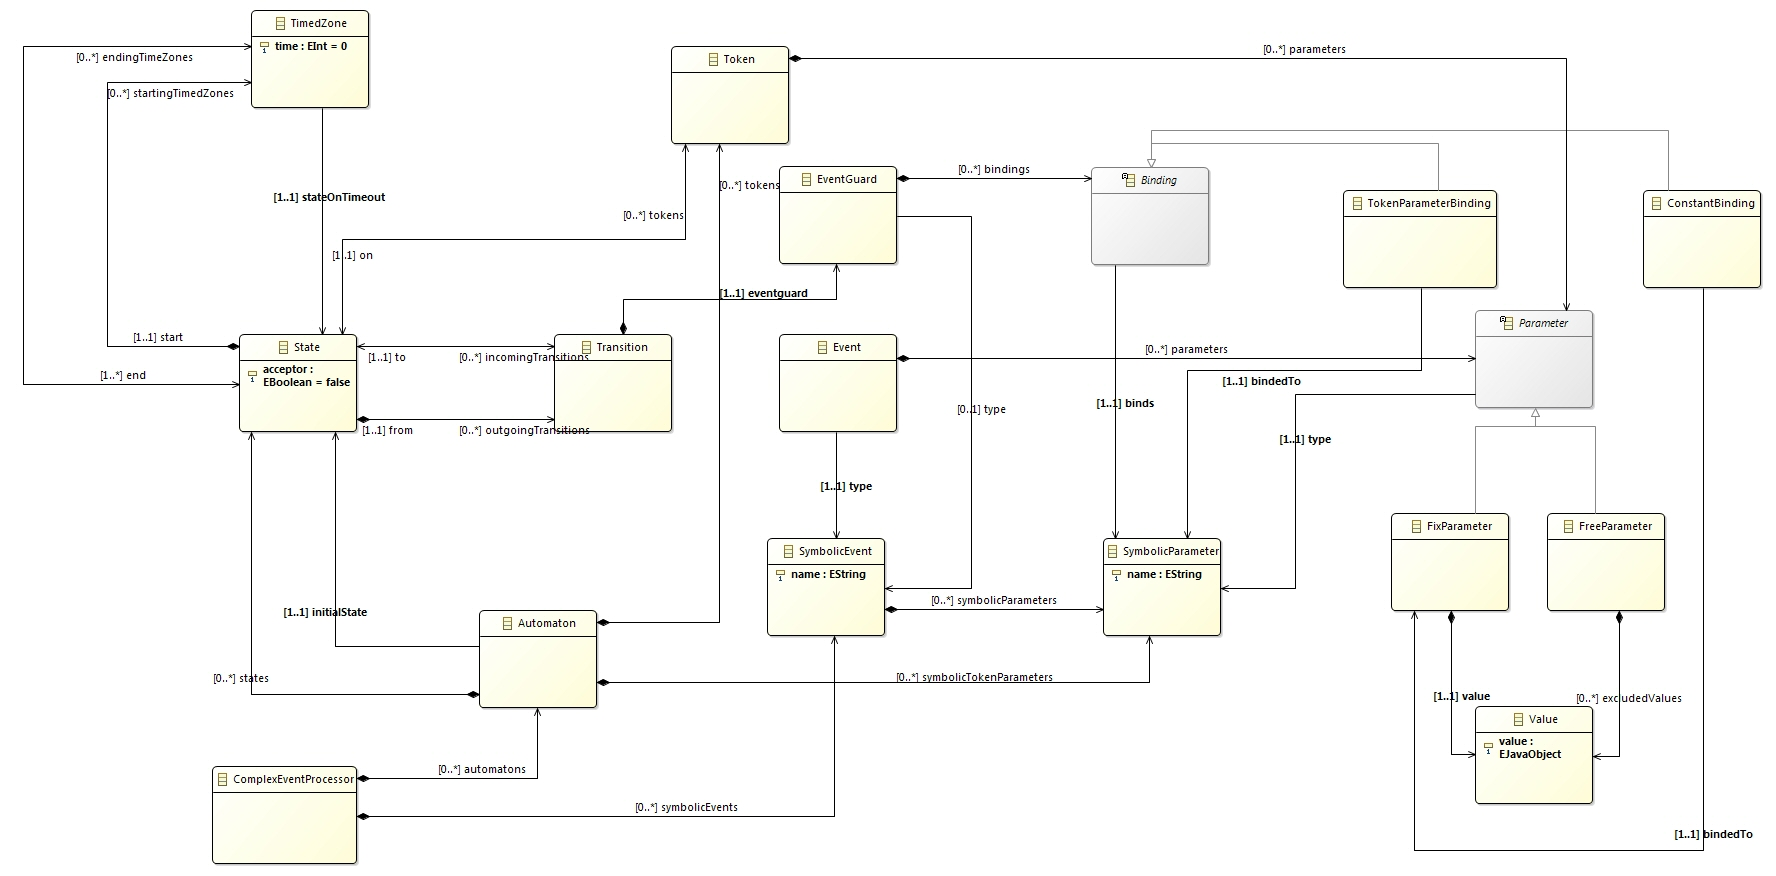
\includegraphics[width=0.9\linewidth]{include/figures/chapter_5/model}
			\caption{Automaton of the file example}
			\label{fig:cep:model}
			\end{figure}
		
			\subsubsection{Basic Automaton}
				The Event Automaton is represented with the State, Transition, and EventGuard classes.
				Every State has a boolean flag 
			\subsubsection{Timing}
			
			\subsubsection{Parameter}
			
			\subsubsection{Binding}
		
		\subsection{Executor}
			The algorithm first searches for all the activated transitions.
			If it finds an activated transition, it iterates over the tokens which are on the state. The first token with matching (non-confronting)
			parameter list will be split to the next state if there are new parameter bindings from the event, or moved if there are no new bindings.
			If a token enters an acceptor state it'll 
			next state 
